\documentclass[10pt,a4paper]{article}
\usepackage[toc,page]{appendix}
\usepackage{authblk} % affiliation
\usepackage[margin=2.4cm]{geometry} % margins
\usepackage{amsmath}
\usepackage{bm} % for bold math
\usepackage{graphicx}
\usepackage[labelfont=bf,nooneline]{caption} % for subfigs % font=small
\usepackage{subcaption} % for subfigs
\usepackage{hyperref} % hyperlinks [colorlinks=true]
\usepackage{booktabs} % spaces between columns
\usepackage{cancel} % MET: $\cancel{\it{E}}_{T}$
\setlength{\tabcolsep}{7pt}

\newcommand{\cc}[1]{\multicolumn{1}{c}{#1}} % centered cell
%\newcommand{\levels}[1]{ \multicolumn{2}{l}{\hspace{-1em}\textbf{#1}}}
\newcommand{\level}[1]{ \multicolumn{5}{l}{\hspace{-1em}\textbf{#1}}}
\newcommand{\T}{\rule{0pt}{2.9ex}}       % Top strut
\newcommand{\B}{\rule[-1.3ex]{0pt}{0pt}} % Bottom strut
\newcommand{\ww}{7.7cm} % width for two figures next to each other
\newcommand{\hh}{1mm} % height between figures above each other
\newcommand{\dd}{-2mm} % distance reduction between one-lined caption and their figure below

\renewcommand{\H}{\text{H}}
\newcommand{\W}{\text{W}}
\renewcommand{\b}{\text{b}}
%\newcommand{\bb}{\text{bb}}
\renewcommand{\tt}{\ensuremath{\text{t}\bar{\text{t}}}}
\newcommand{\di}{$\rightarrow$ bbWW $\rightarrow$ bb$\ell\nu \ell\nu$}
\newcommand{\semi}{$\rightarrow$ bbWW $\rightarrow$ bb$qq\ell\nu$}
\newcommand{\channels}{bbWW $\rightarrow$ bb$\ell\nu\ell\nu$, bb$qq\ell\nu$} % or bbWW $\rightarrow$ bb$qq\ell\nu$ }
\newcommand{\lnu}{\ensuremath{\ell\nu}}
\renewcommand{\ll}{\ensuremath{\ell\ell}}
\newcommand{\sAN}{$\sigma_1$}
\newcommand{\BR}{\mathcal{B}}
\newcommand{\etal}{\emph{et al.}}
\newcommand{\MET}{\ensuremath{\cancel{\it{E}}_{T}}}

\title{Study of Higgs pair production with $\text{H} \rightarrow \text{b}\bar{\text{b}}$ and $\text{H} \rightarrow \text{WW} \rightarrow qq\ell\nu$ for an upgraded CMS detector at the High Luminosity LHC}
\author{A. Hinzmann, B. Kilminster, C. Lange \& I. Neutelings}
\affil{University of Zurich}
\date{December 2015}

% https://twiki.cern.ch/twiki/bin/view/Sandbox/CMSGuidelinesforAuthors
% https://twiki.cern.ch/twiki/bin/view/Sandbox/CMSGuidelinesforAuthors#Symbols
% https://svnweb.cern.ch/cern/wsvn/tdr2/utils/trunk/general/notes_for_authors.pdf
% http://physics.nist.gov/cuu/pdf/sp811.pdf
% http://mirrors.rit.edu/CTAN/macros/latex/contrib/hepnames/hepnames.pdf
% https://twiki.cern.ch/twiki/bin/view/CMS/Internal/PubPreparation

\begin{document}
\maketitle


\abstract{A study of the Higgs boson pair production where one Higgs boson decays into $\text{b}\bar{\text{b}}$ quarks and one into WW bosons in the semi-leptonic final state with a $\text{t}\bar{\text{b}}$ background is presented. The study uses simulated pp collisions at $\sqrt{s} = 14$ TeV in an upgraded CMS detector at the High Luminosity LHC assuming an integrated luminosity $L=3000 \text{ fb}^{-1}$. Kinematic variables are examined for a multivariate analysis with a Boosted Decision Tree.}


%% Introduction
%\section{Introduction}
%This report compares results of selection level cuts of the analysis of HH \di\ with the analysis note by C. Delaere \etal\ \cite{AN} and a new HH \semi\ analysis.





% Samples
\section{Samples}

The signal and background processes are simulated with Monte Carlo samples. These only contain \mbox{$\b\b\W\W \rightarrow \b\b qq\ell\nu$} at generator level, where taus coming from a W-boson are excluded. Both generation and parton shower and hadronization are done in \textsc{Pythia6}. The samples were finally reconstructed with Delphes for the CMS Phase II technical proposal. % reference to technical proposal
Since the jets list in Delphes contains 





% Event selection
\section{Event preselection \& clean-up}
We select from the samples events with at least two b-jets with $p_T > 30$ GeV and $|\eta| < 2.5$, at least four jets with $p_T > 20$ GeV and $|\eta| < 2.5$, exactly one lepton with $p_T > 20$ GeV and $|\eta| < 2.5$ and missing transverse energy \MET $> 20$ GeV.

Further clean-up cuts, $60 \text{ GeV} < M_{\b\b} < 160 \text{ GeV}$ and $\Delta R_{\b\b} < 3 \text{ GeV}$, remove a significant amount of background with out affecting the signal too much.


% FIGURE: M_bb and DeltaR_bb before clean-up
\begin{figure*}[h]
    % fig a
    \begin{minipage}[h!]{\ww}
      \centering
      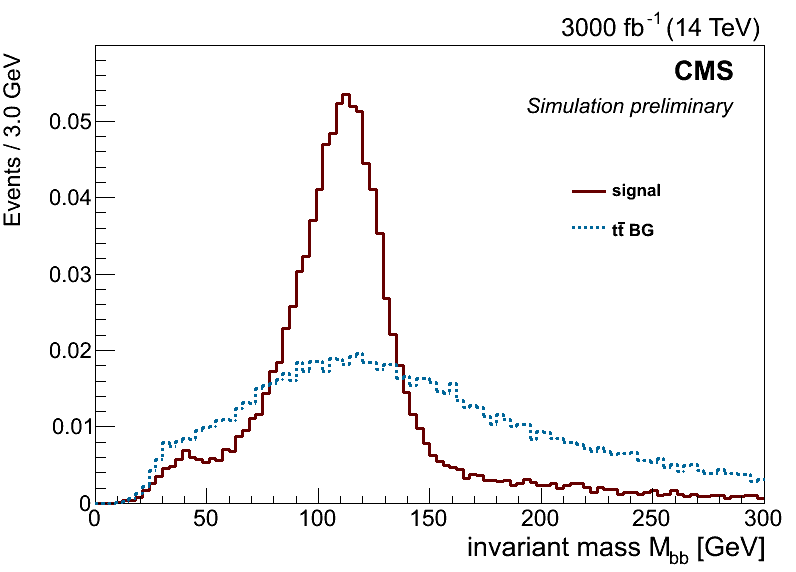
\includegraphics[width=\ww]{figs/M_bb_closest_stage1.png}
    \end{minipage}
%    \hspace{\w}
    % fig b
    \begin{minipage}[h!]{\ww}
      \centering
      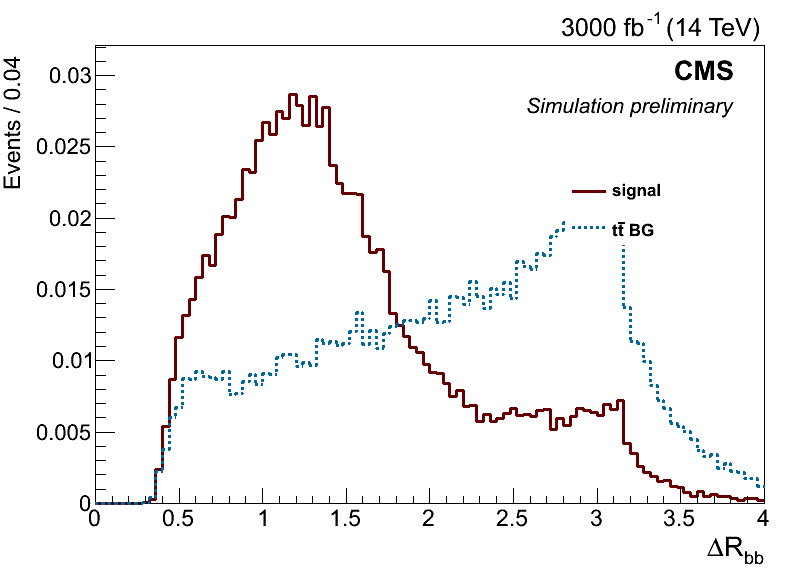
\includegraphics[width=\ww]{figs/DeltaR_bb1_stage1.png}
    \end{minipage}
  \vspace{\dd}
  \caption{$M_\text{bb}$ and $\Delta R_\text{bb}$ before clean-up.} \label{multi}
\end{figure*}



The branching ratios are found using
\begin{align*}
    \mathcal{B}(\text{HH $\rightarrow$ bbWW})
        &= 2\mathcal{B}(\text{H $\rightarrow$ bb})
            \mathcal{B}(\text{H $\rightarrow$ WW})
        \simeq 0.248 \\
    \mathcal{B}(\text{\tt\ $\rightarrow$ bWbW})
        &= \mathcal{B}(\text{t $\rightarrow$ bW})^2
        \simeq 0.997 \\
%              0,9966 CDF 2014
%              0,8281 PDG 2014
%    \mathcal{B}(\text{WW $\rightarrow$ \lnu\lnu})
%        &= \mathcal{B}(\text{W $\rightarrow$ \lnu})^2
%        \simeq 0.046 \\
    \mathcal{B}(\text{WW $\rightarrow qq$\lnu})
        &= 2\mathcal{B}(\text{W $\rightarrow$ $qq$})
            \mathcal{B}(\text{W $\rightarrow$ \lnu})
        \simeq 0.288
\end{align*}
with numbers from \cite{BR_HH}, \cite{BR_tt} and \cite{BR_W}:
\begin{align*}
%    \mathcal{B}(\text{HH $\rightarrow$ bbWW $\rightarrow$ bb\lnu\lnu})
%         &\simeq 0.011\\
%        &= 2\mathcal{B}(\text{H $\rightarrow$ bb})
%            \mathcal{B}(\text{H $\rightarrow$ WW})
%            \mathcal{B}(\text{W $\rightarrow \ell\nu$})^2 \\
    \mathcal{B}(\text{HH $\rightarrow$ bbWW $\rightarrow$ bb$qq$\lnu})
         &\simeq 0.072\\
%        &= 2\mathcal{B}(\text{H $\rightarrow$ bb})
%            \mathcal{B}(\text{H $\rightarrow$ WW})
%            *2\mathcal{B}(\text{W $\rightarrow$ qq})
%            \mathcal{B}(\text{W $\rightarrow \ell\nu$}) \\
%    \mathcal{B}(\text{\tt\ $\rightarrow$ bbWW $\rightarrow$ bb$qq$\lnu\lnu})
%         &\simeq 0.045\\
%        &=  \mathcal{B}(\text{t $\rightarrow$ bW})^2
%            \mathcal{B}(\text{W $\rightarrow \ell\nu$})^2 \\
    \mathcal{B}(\text{\tt\ $\rightarrow$ bbWW $\rightarrow$ bb$qq$\lnu})
         &\simeq 0.287
%        &=  \mathcal{B}(\text{t $\rightarrow$ bW})^2
%            *2\mathcal{B}(\text{W $\rightarrow$ qq})
%            \mathcal{B}(\text{W $\rightarrow \ell\nu$}) \\
\end{align*}



\begin{table}[h]
	\centering
	\caption{Cross sections at NNLO and $\sqrt{s}=14$ TeV \cite{sigma_HH}\cite{sigma_tt}, branching ratios $\BR$ (excluding W $\rightarrow \tau\bar{\tau}$) \cite{BR_HH}\cite{BR_tt}\cite{BR_W} and number of Monte Carlo events per process in the samples.} %\vspace{2mm}
	\label{sigma}
	\begin{tabular}{@{\;}lccc@{\;}}
	\toprule
	process      & $\sigma\BR$ [fb] & branching ratio $\BR$ & number of MC events \\
	\midrule
	\textbf{HH}  & \textbf{40}      &           & \\ %\textbf{979 907} \\
	HH \semi     &        2.88      &   0.072   &  166 483  \\
	HH \di       &        0.44      &   0.011   &   22 812  \\
	\textbf{\tt} & \textbf{984 500} &           & \\ %\textbf{499 600} \\
	\tt \semi    &     282 552      &   0.287   &  164 661  \\
	\tt \di      &      44 303      &   0.045   &   22 546  \\
	\bottomrule
	\end{tabular}
\end{table}



\begin{table}[h]
	%\small
	\centering
	\caption{Significance $P=S/(1+\sqrt{B})$ and yields $S:=N(\H\H)$ and $B:=N(\tt)$ with NNLO cross sections at $\sqrt{s}=14$ TeV and with integrated luminosity $L = 3000 \text{ fb}^{-1}$.} %\vspace{5pt}  %, cross sections \sAN\ from Table \ref{sigma_AN}
%	\label{comparison}
	\begin{tabular}{@{\;}lrrr@{\;}}
	
	\toprule
	Selection level & \cc{$P$} & \cc{$S$} & \cc{$B$} \\
	\midrule
	Initial $\text{bbWW} \rightarrow \text{bb}qq\ell\nu$ sample
		& 0.297 &   8640  & 847 654 500  \\
	Selection
 		& 0.109 &   1496  & 189 235 942  \\
	Clean-up
 		& 0.130 &   1153  &  78 762 511  \\
	\bottomrule
	
	\end{tabular}
\end{table}









% Cross section
\section{Multivariate analysis}


The TMVA's boosted decision tree (BDT) is used for the multivariate analysis. The following are input variables for the BDT:
% variable list
$p_T^\text{bb}$ of the two b-tagged jets,
$p_T^{jj}$ of the two leading ``light'' jets,
$p_T^\ell$ of the leading lepton,
\MET,
$p_T^\text{bb}$,
$p_T^{\text{b}_2\ell}$,
$p_T^{j_1\ell}$,
$\Delta R_{j_1\ell}$,
$\Delta R_{j_2\ell}$,
$\Delta R_{\text{b}_1\ell}$,
$\Delta R_{\text{b}_2\ell}$,
$\Delta R_{\b\b}$,
$\Delta R_{jj}$,
$\Delta R_{jj,l}$,
$\Delta R_{jj,\text{b}_1}$,
%$\Delta\phi_{l,\text{\MT}}$,
$\Delta\phi_{j_1\ell\text{,bb}}$,
$M_{\b\b}$,
$M_{jjl}$,
$M_{jj,\text{b}_1}$,
$M_{jj,\text{b}}$,
$M_{\text{b}_2\text{\lnu}}$.
$M_{\text{b}_2\text{\l}}$ and
$M_T^{\ell\nu}$.
% further explanation
Here $j_1$ denotes the light jet closest to the lepton, and $j_2$ the second closest, while $\text{b}_1$ denotes the b-tagged jet farthest to the lepton and $\text{b}_2$ the second farthest. In case of more than two b-jets, the b-jet pair closest in $\Delta R_{\b\b}$ is used for $M_{\b\b}$ and other b-tagged jets are then regarded as light jets.
% top mass reconstructions
To exploit the top mass, two invariant masses reconstruct a leptonic and hadronic top as follows: the two leading jets and closest b-jet second closest to the lepton (i.e. $b_1$ in case of only two b-tagged jets) form $M_{jj,\text{b}_1}$ and the lepton, reconstructed neutrino and b-jet closest to the lepton make $M_{\text{b}_2\text{\lnu}}$. The neutrino here is reconstructed assuming its transverse momentum $p^\nu_T$ is given by the missing transverse energy and its longitudinal component $p^\nu_z$ is (the real part of) the solution of $M_\text{W}^2 = (p_\ell + p_\nu)^2$.
% transverse mass
The transverse mass $M_T^{\ell\nu}$ is defined as
\begin{equation} \label{MT}
	M_T^{\ell\nu} = \sqrt{ 2 p_T^\ell \text{\MET} ( 1 - \cos \Delta \phi_{\ell,\text{\MET}} )}.
\end{equation}
All variables are shown Figs. \ref{vars1}-\ref{vars8}.

The final BDT output and background rejection versus signal efficiency of the test sample is shown in Fig. \ref{BDT}. A cut is made at 0.44, yielding a significance of $P=0.37$ %(see Eq. \eqref{P})
, 27 signal events and 5153 background events at an integrated lumininosity $L = 3000 \text{ fb}^{-1}$.



%\begin{table}[p]
%	\centering
%	\caption{Cross sections for their Monte Carlo samples listed in the analysis note by C. Deleare \etal\ \cite{AN}.} \vspace{5pt} %and \sAN\ from Eq. \eqref{sf} with a filter efficiency $e=1$ for HH and $e=0.37$ for \tt\ to account for cuts at generator level.
%	\label{sigma_AN}
%	\begin{tabular}{@{}lcccc@{}}
%	\toprule
%	process            & $\sigma_\text{LO}$ [fb] & $k_\text{NNLO}$ & number of MC events \\
%	\midrule
%	HH \di             &  0.163  &   2.3   & 1.1M \\
%	\tt\ full leptonic &  9030   &  1.85   & 4.8M \\
%%	HH \di             &  0.163  &   2.3   &  33.2   & 1.1M \\
%%	\tt\ full leptonic &  9030   &  1.85   & 994 493 & 4.8M \\
%	\bottomrule
%	\end{tabular}
%\end{table}
%
%
%\begin{table}[p]
%	\centering
%	\caption{Number of MC events in our sample at each level of selection.} \vspace{5pt}
%	\label{raw}
%	\begin{tabular}{@{\quad}lrrrr@{}}
%	
%	\toprule
%	               & \multicolumn{2}{c}{dileptonic final state} & \multicolumn{2}{c}{semileptonic final state} \\
%	\cmidrule(r){2-3} \cmidrule(r){4-5}
%	selection level                      &  signal  & background &  signal  & background \\
%	\midrule
%% without taus in sample
%	\channels				             &  22812  &  22546 & 166483 & 164661 \\
%	Generator level filter on background &  22812  &   8339 & 166483 & 137880 \\
%	Selection                            &   2571  &   1636 &  28821 &  36760 \\
%	Clean-up                             &   2066  &    280 &  22225 &  15300 \\
%% with taus in sample
%%	Sample without any cuts      &  51464  &  50789 & 214888 & 211952 \\
%%	Gen level cuts on background &  51464  &  18899 & 214888 & 101940 \\
%%	Selection                    &   3181  &   2023 &  26511 &  20848 \\
%%	Clean-up                     &   2499  &    331 &  20634 &   9428 \\
%	\bottomrule
%	
%	\end{tabular}
%\end{table}


% FIGURE: sketch
\begin{figure*}[h]
    % fig a
    \begin{minipage}[h!]{\ww}
      \centering
      \includegraphics[width=7cm]{sketch/sketch_HH.png}
    \end{minipage}
%    \hspace{\w}
    % fig b
    \begin{minipage}[h!]{\ww}
      \centering
      \includegraphics[width=7cm]{sketch/sketch_tt.png}
    \end{minipage}
%  \vspace{-6mm}
  \caption{Sketch of a boosted Higgs boson pair and a boosted \tt\ pair.} \label{sketch}
\end{figure*}


% FIGURE: multicplicities
\begin{figure*}[h]
    % fig a
    \begin{minipage}[h!]{\ww}
      \centering
      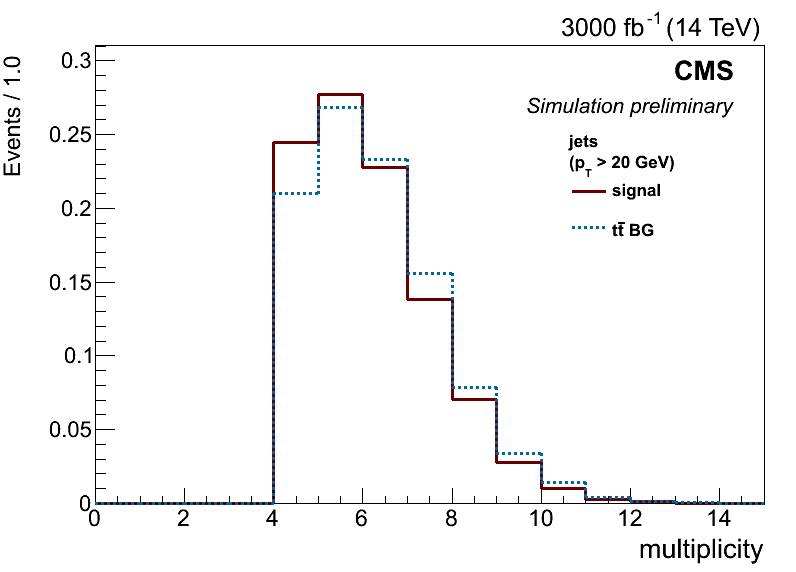
\includegraphics[width=\ww]{figs/Njets20.png}
    \end{minipage}
%    \hspace{\w}
    % fig b
    \begin{minipage}[h!]{\ww}
      \centering
      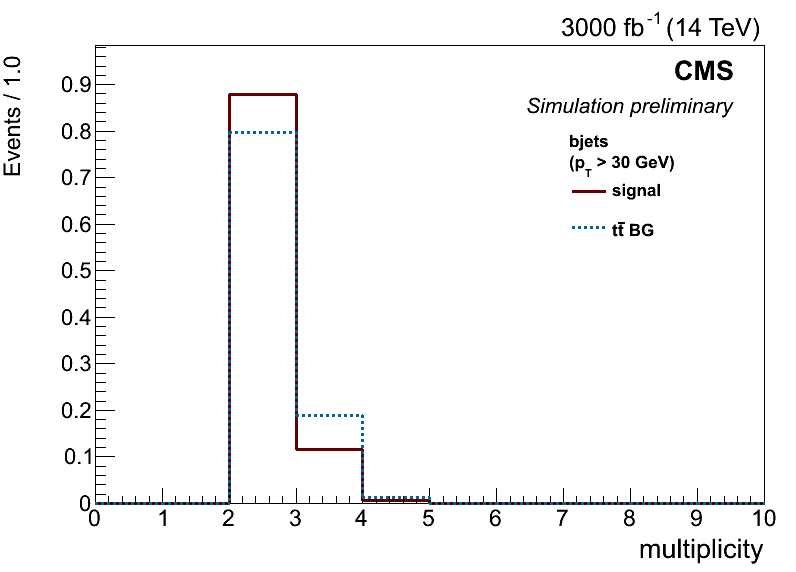
\includegraphics[width=\ww]{figs/Nbjets30.png}
    \end{minipage}
  \vspace{\dd}
  \caption{Multiplicities of $p_T>20$ GeV jets and $p_T>30$ GeV.} \label{multi}
\end{figure*}


% FIGURE: p_T lepton, MET
\begin{figure*}[h]
    % fig a
    \begin{minipage}[h!]{\ww}
      \centering
      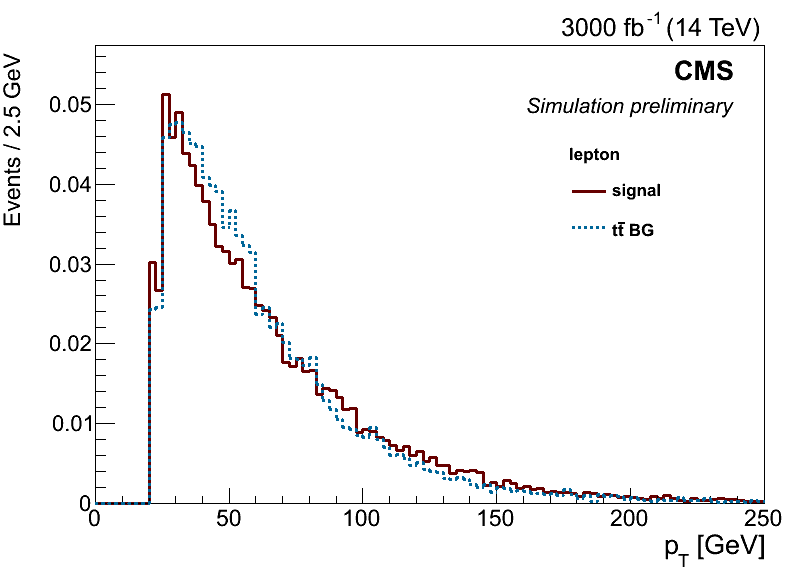
\includegraphics[width=\ww]{figs/leptonPt.png}
    \end{minipage}
%    \hspace{\wb}
    % fig b
    \begin{minipage}[h!]{\ww}
      \centering
      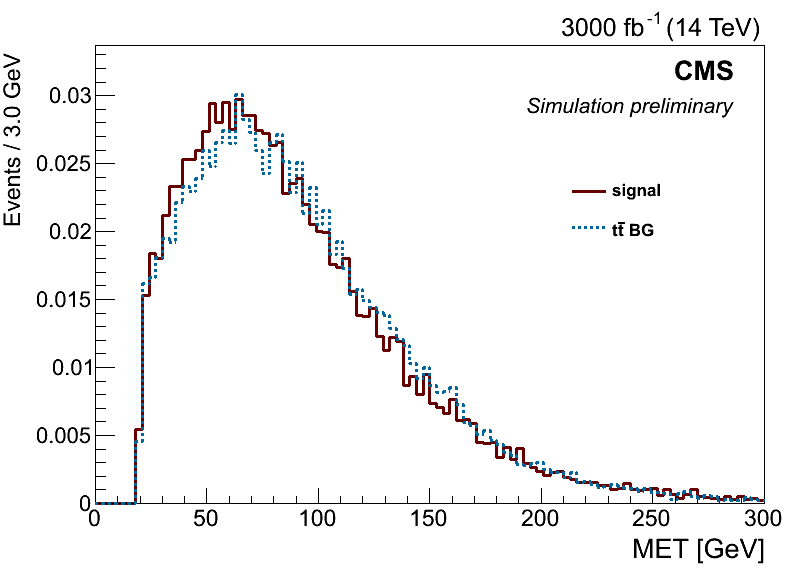
\includegraphics[width=\ww]{figs/MET.png}
    \end{minipage}
  \vspace{\dd}
  \caption{Variables distribution of HH (red) and \tt\ (blue) for the neural network: transverse momentum $p_T$ of the lepton and missing transverse energy \MET.} \label{vars1}
\end{figure*}


%% FIGURE
%\begin{figure*}[h]
%	
%  % SUBFIGURES
%  \begin{subfigure}[b]{17cm}
%    % fig a
%    \begin{minipage}[h!]{\ww}
%      \centering
%      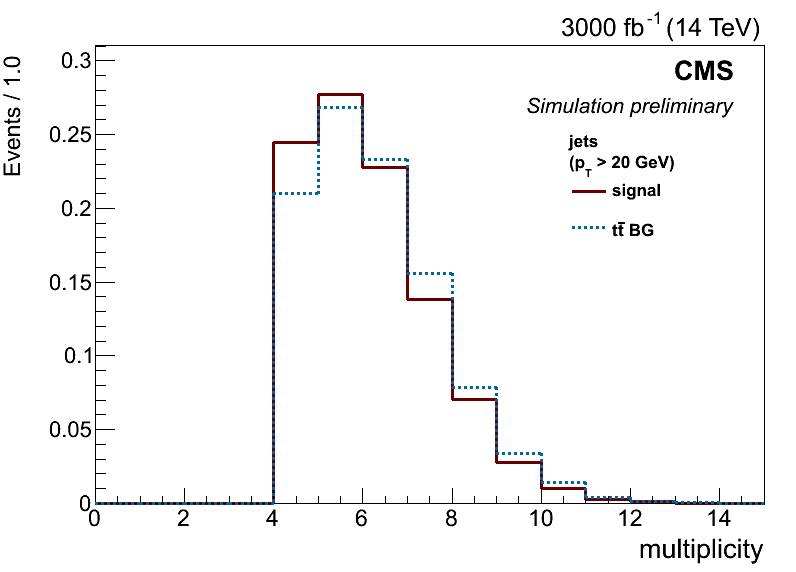
\includegraphics[width=\ww]{figs/Njets20.png}
%    \end{minipage}
%%    \hspace{\w}
%    % fig b
%    \begin{minipage}[h!]{\ww}
%      \centering
%      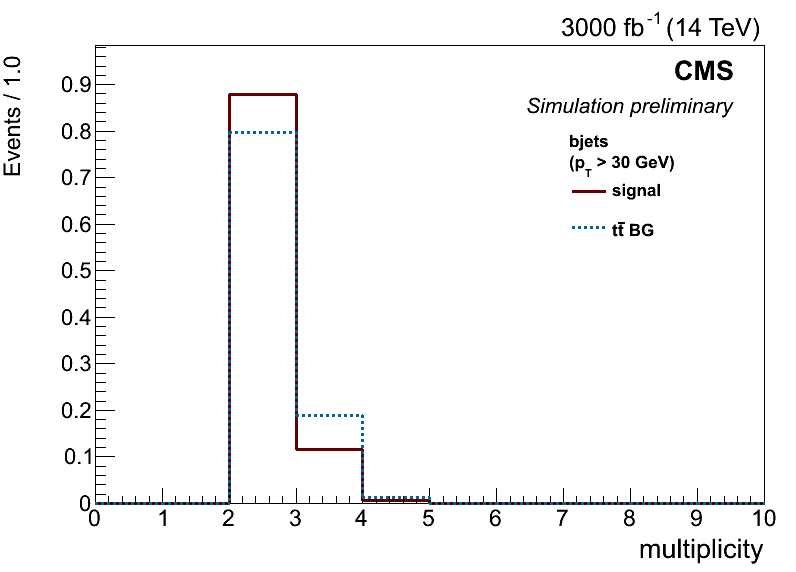
\includegraphics[width=\ww]{figs/Nbjets30.png}
%    \end{minipage}
%  \end{subfigure}
%
%  % SUBFIGURES
%  \begin{subfigure}[b]{17cm}
%    % fig a
%    \begin{minipage}[h!]{\ww}
%      \centering
%      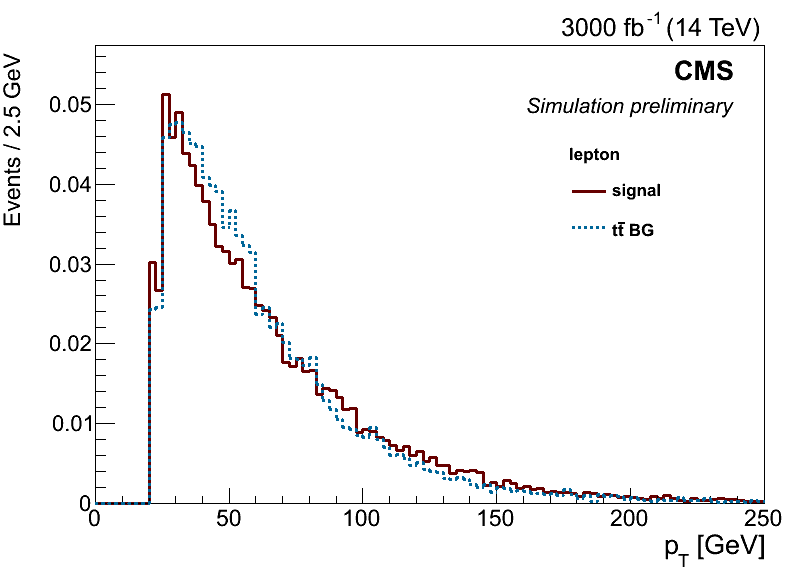
\includegraphics[width=\ww]{figs/leptonPt.png}
%    \end{minipage}
%%    \hspace{\wb}
%    % fig b
%    \begin{minipage}[h!]{\ww}
%      \centering
%      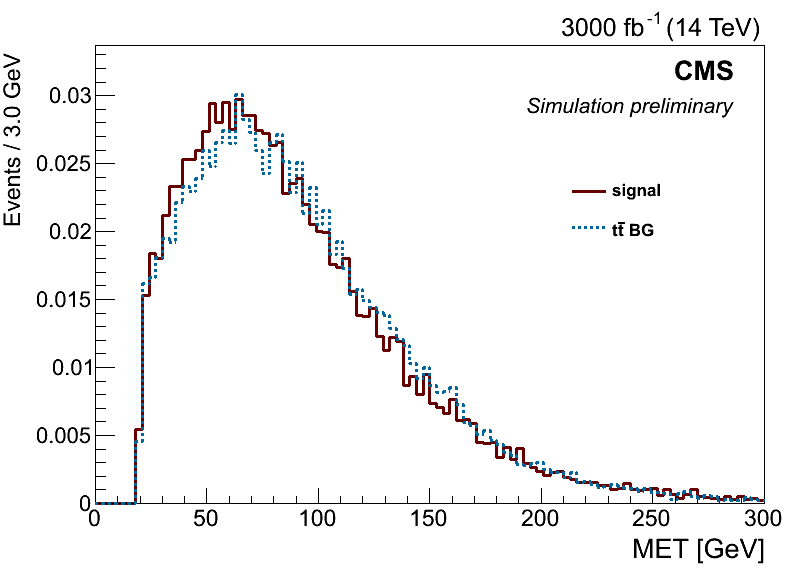
\includegraphics[width=\ww]{figs/MET.png}
%    \end{minipage}
%  \end{subfigure}	
%  \vspace{\dd}
%  \caption{Variables distribution of HH (red) and \tt\ (blue) for the neural network: $p_T>20$ GeV jet multiplicity, $p_T>30$ GeV b-jet multiplicity, transverse momentum $p_T$ of the lepton and missing transverse energy \MET.} \label{vars1}
%
%\end{figure*}



% FIGURE: p_T jets and b-jets
\begin{figure*}[h]
	
  % SUBFIGURES
  \begin{subfigure}[b]{17cm}
    % fig a
    \begin{minipage}[h!]{\ww}
      \centering
      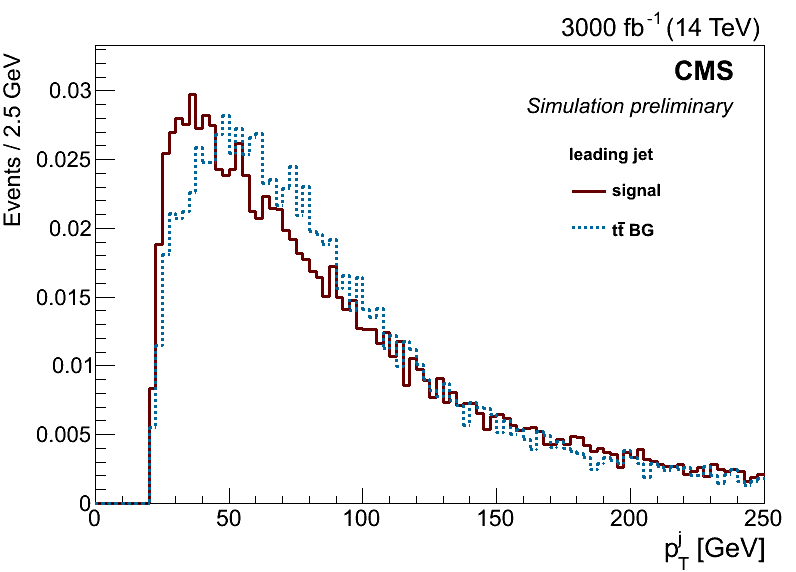
\includegraphics[width=\ww]{figs/jet1Pt.png}
    \end{minipage}
%    \hspace{\w}
    % fig b
    \begin{minipage}[h!]{\ww}
      \centering
      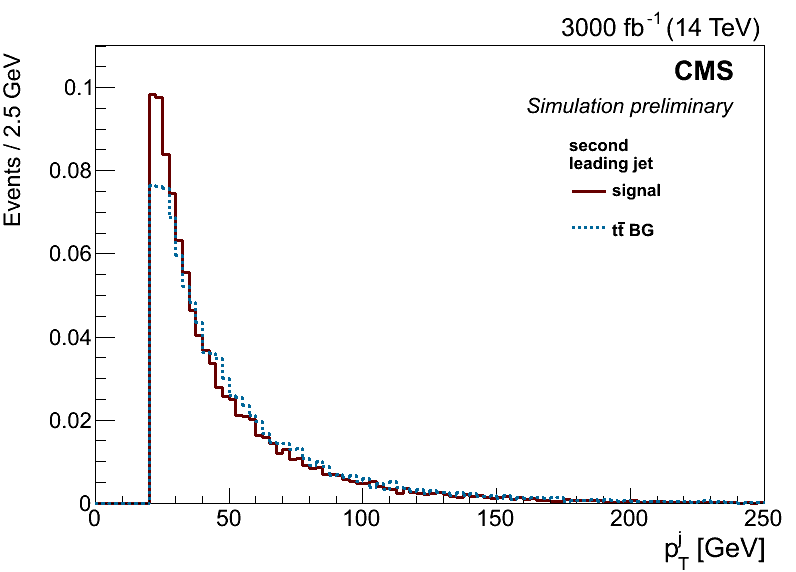
\includegraphics[width=\ww]{figs/jet2Pt.png}
    \end{minipage}
  \end{subfigure}

  % SUBFIGURES
  \begin{subfigure}[b]{17cm}
    % fig a
    \begin{minipage}[h!]{\ww}
      \centering
      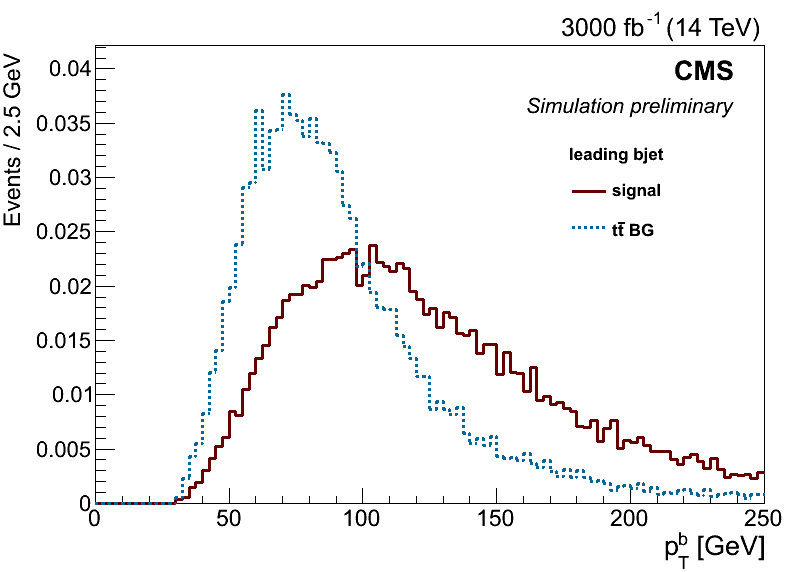
\includegraphics[width=\ww]{figs/bjet1Pt.png}
    \end{minipage}
%    \hspace{\wb}
    % fig b
    \begin{minipage}[h!]{\ww}
      \centering
      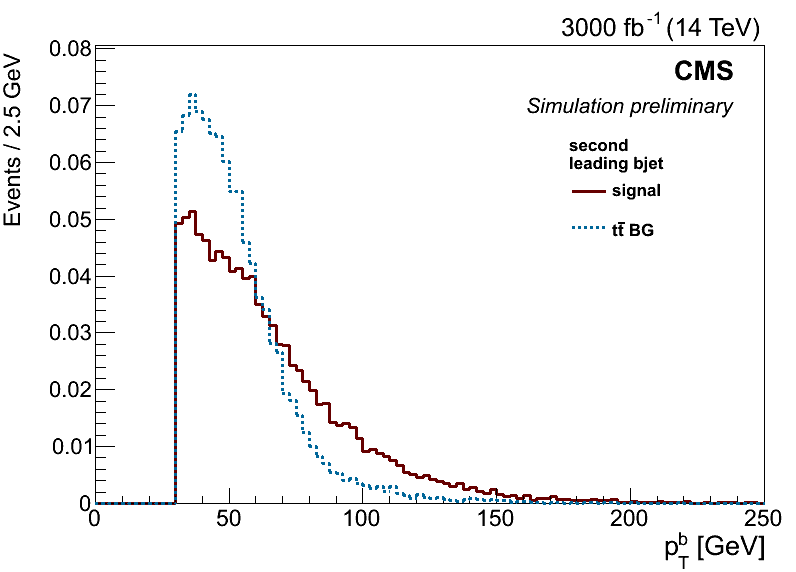
\includegraphics[width=\ww]{figs/bjet2Pt.png}
    \end{minipage}
  \end{subfigure}	
  \vspace{\dd}
  \caption{Variables distribution of HH (red) and \tt\ (blue) for the neural network: transverse momentum $p_T$ for the two leading jets and two leading b-jets.} \label{vars2}

\end{figure*}



% FIGURE: p_T bb, jj, j1l and DeltaPhi_j1lbb
\begin{figure*}[h]
	
  % SUBFIGURES
  \begin{subfigure}[b]{17cm}
    % fig a
    \begin{minipage}[h!]{\ww}
      \centering
      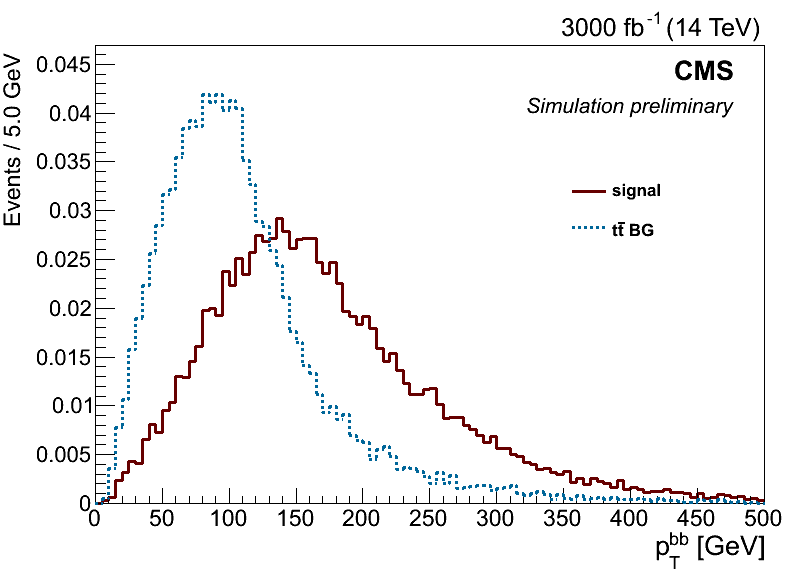
\includegraphics[width=\ww]{figs/Pt_bb.png}
    \end{minipage}
%    \hspace{\w}
    % fig b
    \begin{minipage}[h!]{\ww}
      \centering
      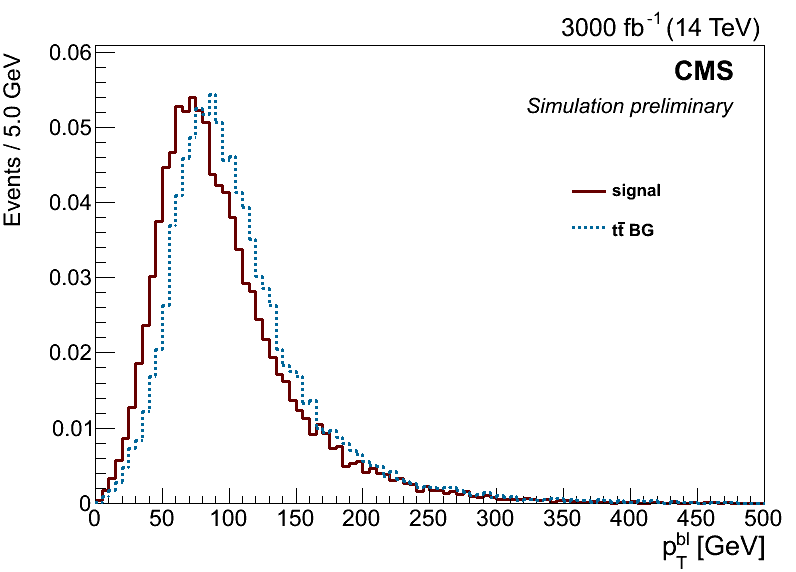
\includegraphics[width=\ww]{figs/Pt_bl.png}
    \end{minipage}
  \end{subfigure}

  % SUBFIGURES
  \begin{subfigure}[b]{17cm}
    % fig a
    \begin{minipage}[h!]{\ww}
      \centering
      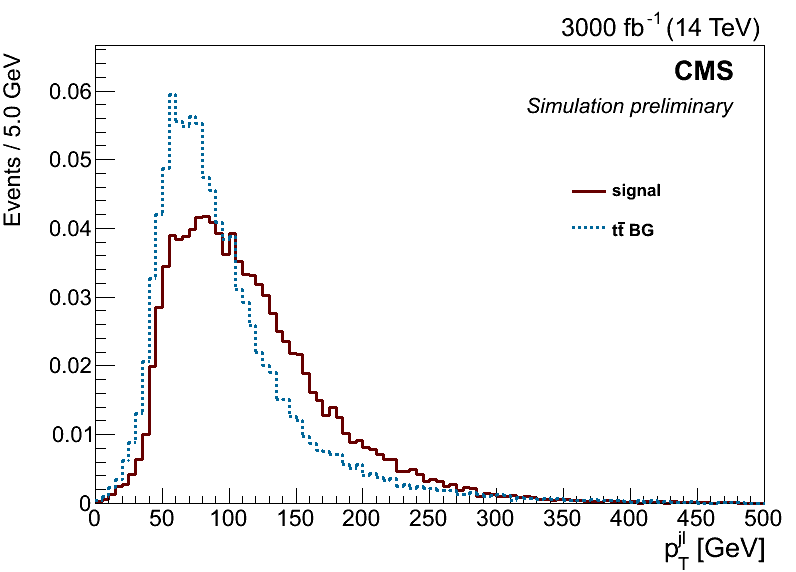
\includegraphics[width=\ww]{figs/Pt_j1l.png}
    \end{minipage}
%    \hspace{\wb}
    % fig b
    \begin{minipage}[h!]{\ww}
      \centering
      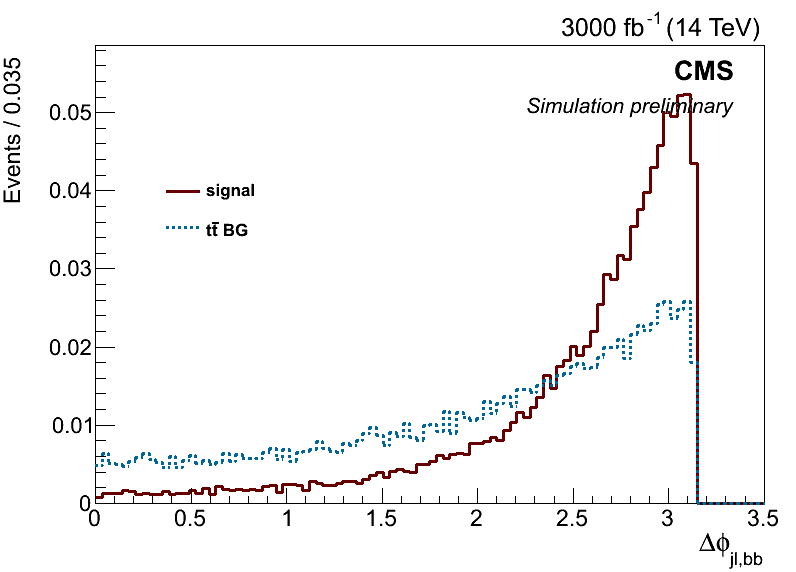
\includegraphics[width=\ww]{figs/DeltaPhi_j1lbb.png}
    \end{minipage}
    \hspace{9mm}
  \end{subfigure}	
  \vspace{\dd}
  \caption{Variables distribution of HH (red) and \tt\ (blue) for the neural network: $p_T^\text{bb}$, $p_T^{jj}$, $p_T^{j_1\ell}$ and $\Delta\phi_{j_1\ell\text{,bb}}$.} \label{vars4}

\end{figure*}



% FIGURE: DeltaR j1l, j2l, b1l, b2l
\begin{figure*}[h]
	
  % SUBFIGURES
  \begin{subfigure}[b]{17cm}
    % fig a
    \begin{minipage}[h!]{\ww}
      \centering
      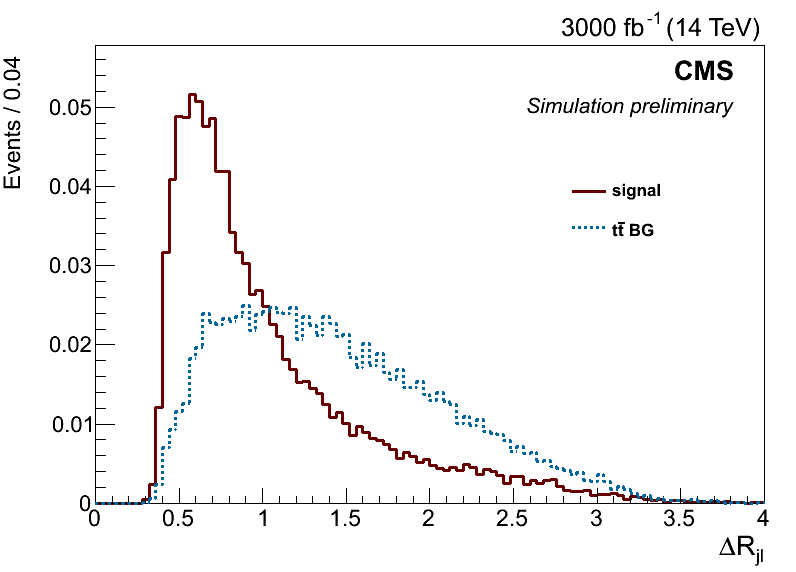
\includegraphics[width=\ww]{figs/DeltaR_j1l.png}
    \end{minipage}
%    \hspace{\w}
    % fig b
    \begin{minipage}[h!]{\ww}
      \centering
      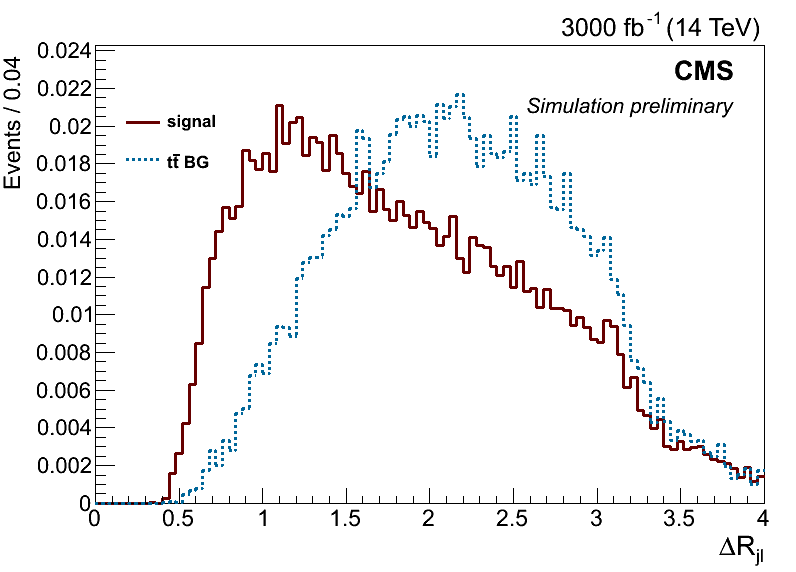
\includegraphics[width=\ww]{figs/DeltaR_j2l.png}
    \end{minipage}
  \end{subfigure}

  % SUBFIGURES
  \begin{subfigure}[b]{17cm}
    % fig a
    \begin{minipage}[h!]{\ww}
      \centering
      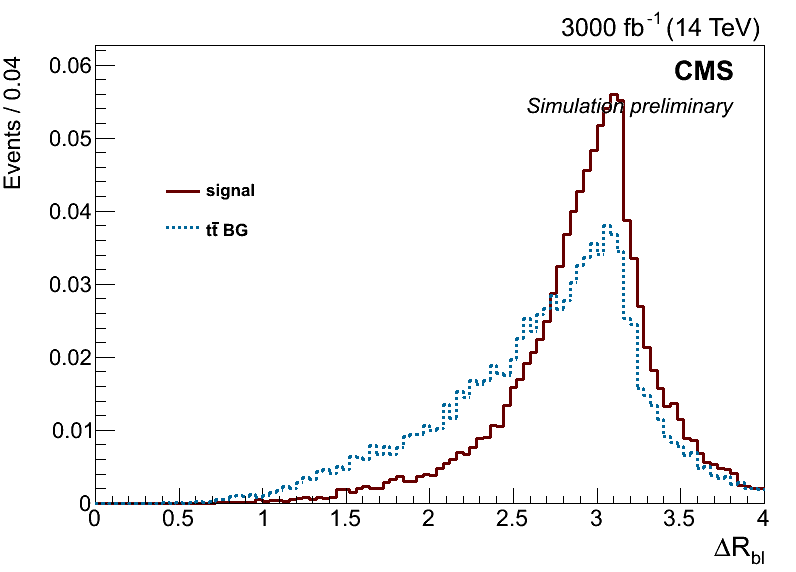
\includegraphics[width=\ww]{figs/DeltaR_b1l.png}
    \end{minipage}
%    \hspace{\wb}
    % fig b
    \begin{minipage}[h!]{\ww}
      \centering
      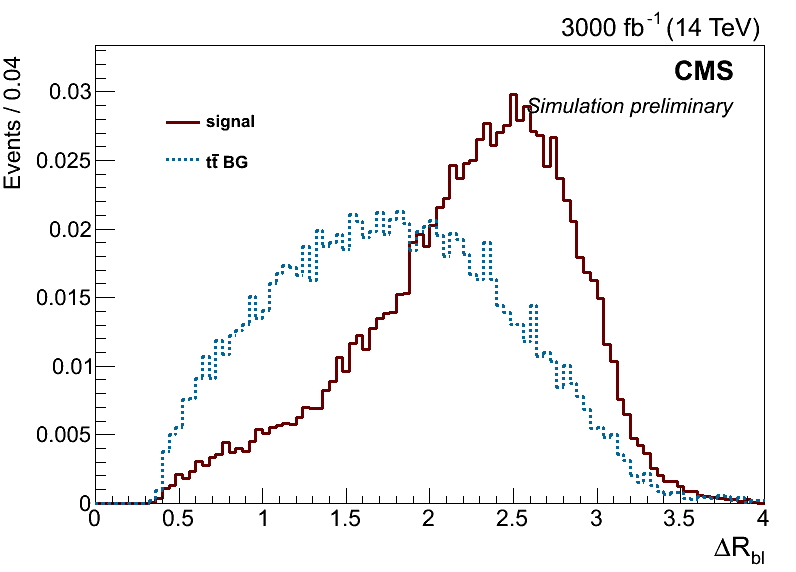
\includegraphics[width=\ww]{figs/DeltaR_b2l.png}
    \end{minipage}
    \hspace{9mm}
  \end{subfigure}	
  \vspace{\dd}
  \caption{Variables distribution of HH (red) and \tt\ (blue) for the neural network: $\Delta R_{j_1\ell}$, $\Delta R_{j_2\ell}$, $\Delta R_{b_1\ell}$ and $\Delta R_{b_2\ell}$.} \label{vars5} %between the lepton and the two closest light jets and between the lepton and two farthest b-jets

\end{figure*}



% FIGURE: DeltaR bb, jj, jjb, jjl
\begin{figure*}[h]
	
  % SUBFIGURES
  \begin{subfigure}[b]{17cm}
    % fig a
    \begin{minipage}[h!]{\ww}
      \centering
      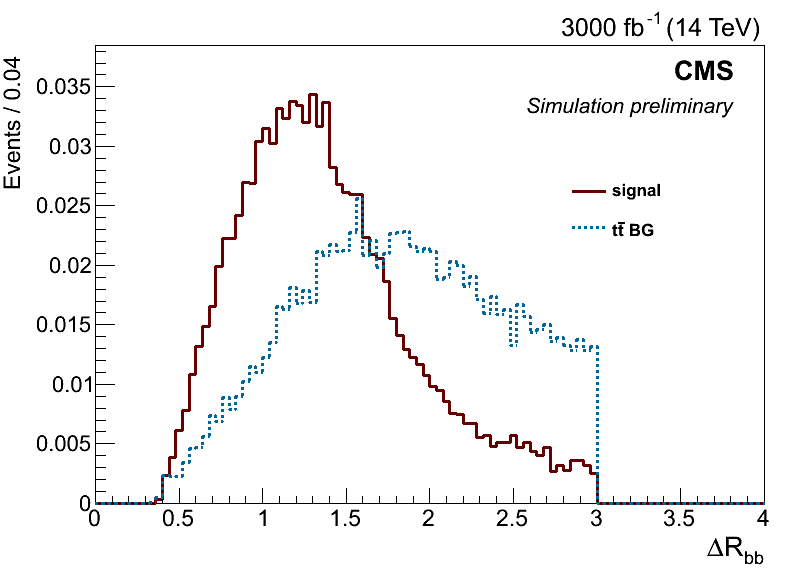
\includegraphics[width=\ww]{figs/DeltaR_bb1.png}
    \end{minipage}
%    \hspace{\w}
    % fig b
    \begin{minipage}[h!]{\ww}
      \centering
      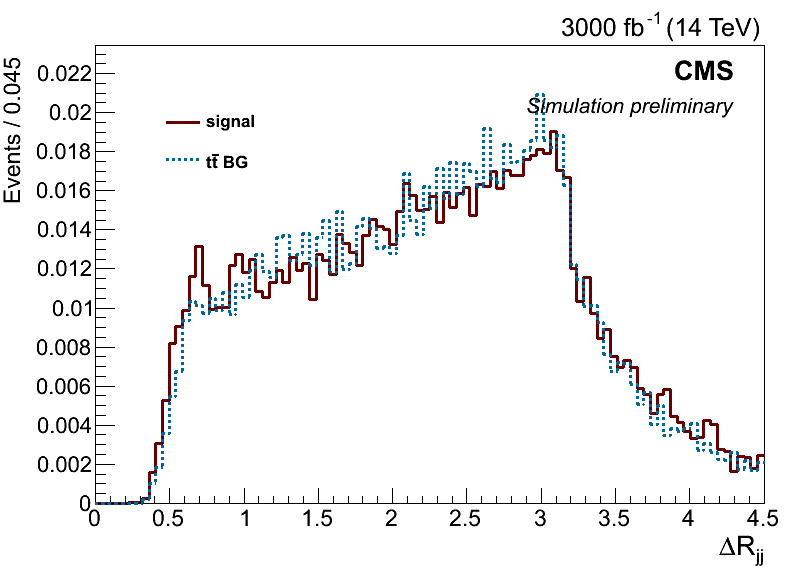
\includegraphics[width=\ww]{figs/DeltaR_jj.png}
    \end{minipage}
  \end{subfigure}

  % SUBFIGURES
  \begin{subfigure}[b]{17cm}
    % fig a
    \begin{minipage}[h!]{\ww}
      \centering
      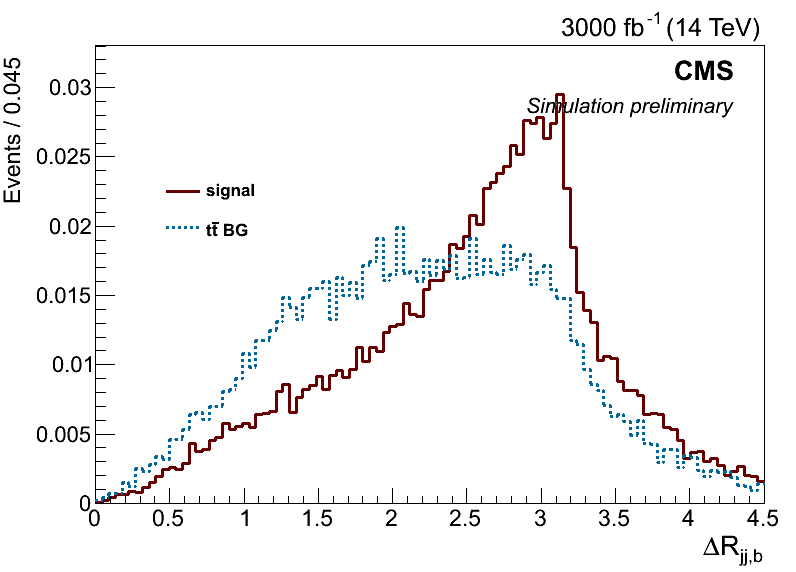
\includegraphics[width=\ww]{figs/DeltaR_jjb.png}
    \end{minipage}
%    \hspace{\wb}
    % fig b
    \begin{minipage}[h!]{\ww}
      \centering
      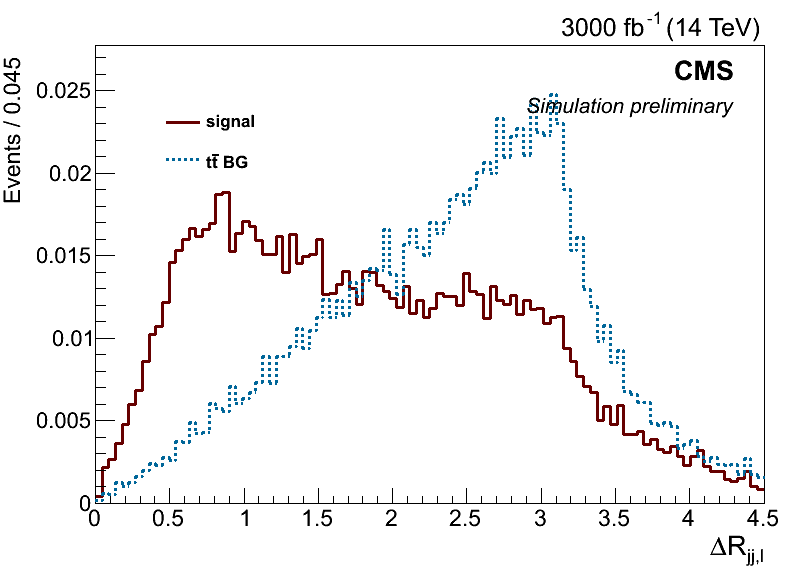
\includegraphics[width=\ww]{figs/DeltaR_jjl.png}
    \end{minipage}
  \end{subfigure}	
  \vspace{\dd} 
  \caption{Variables distribution of HH (red) and \tt\ (blue) for the neural network: $\Delta R_{bb}$, $\Delta R_{jj}$, $\Delta R_{jj,b_1}$ and $\Delta R_{jj,\ell}$.} \label{vars6}

\end{figure*}



% FIGURE: M bb, jjl, jjb, b2lnu
\begin{figure*}[h]
	
  % SUBFIGURES
  \begin{subfigure}[b]{17cm}
    % fig a
    \begin{minipage}[h!]{\ww}
      \centering
      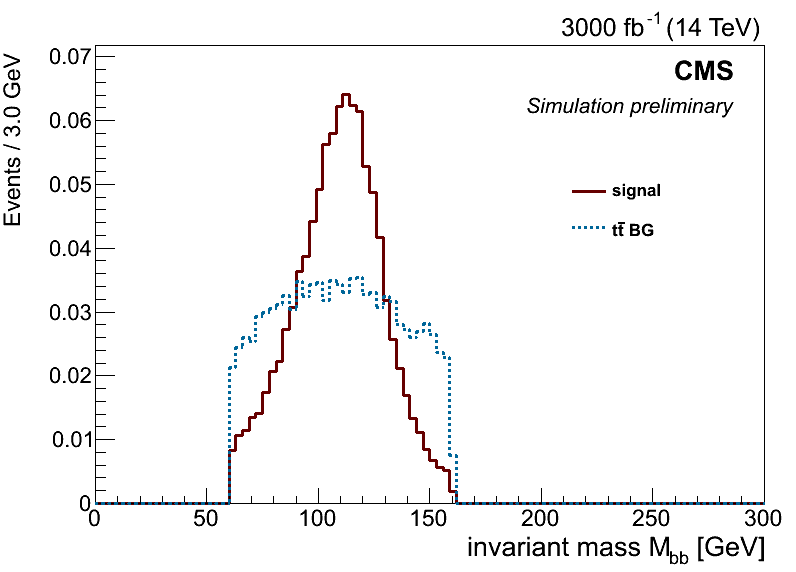
\includegraphics[width=\ww]{figs/M_bb_closest.png}
    \end{minipage}
%    \hspace{\w}
    % fig b
    \begin{minipage}[h!]{\ww}
      \centering
      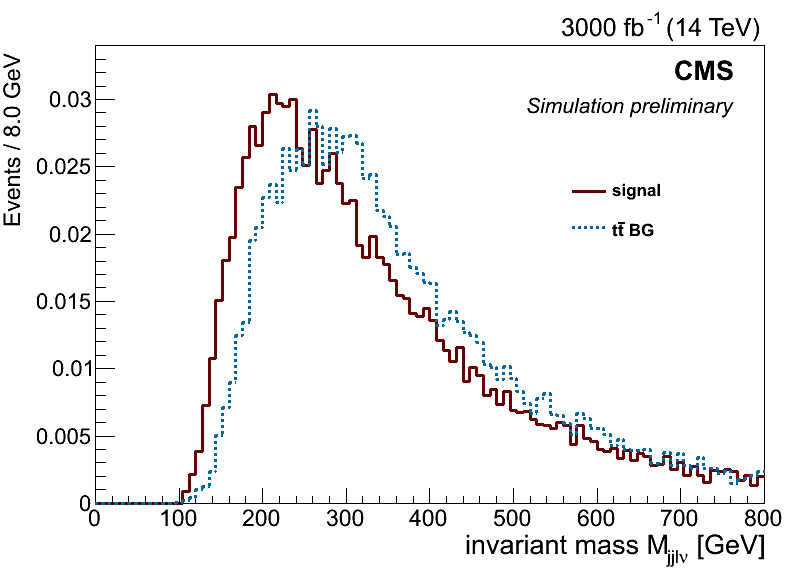
\includegraphics[width=\ww]{figs/M_jjlnu.png}
    \end{minipage}
  \end{subfigure}

  % SUBFIGURES
  \begin{subfigure}[b]{17cm}
    % fig a
    \begin{minipage}[h!]{\ww}
      \centering
      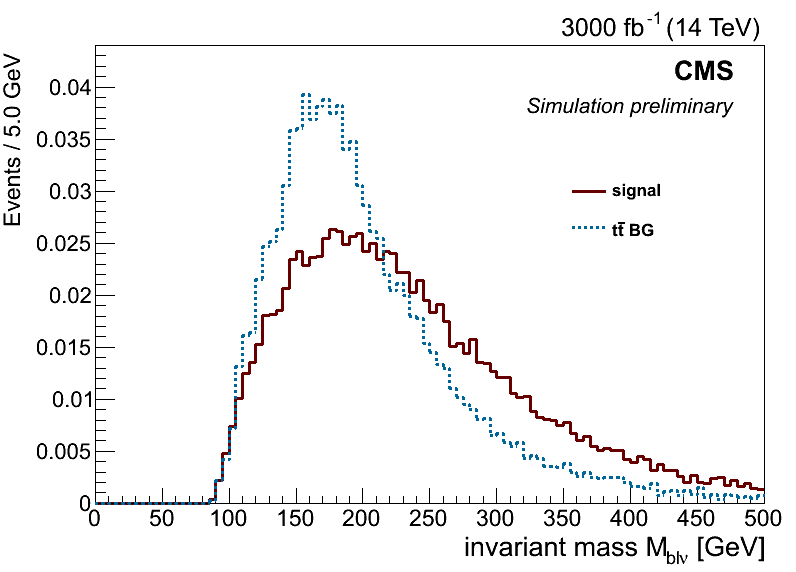
\includegraphics[width=\ww]{figs/M_blnu.png}
    \end{minipage}
%    \hspace{\wb}
    % fig b
    \begin{minipage}[h!]{\ww}
      \centering
      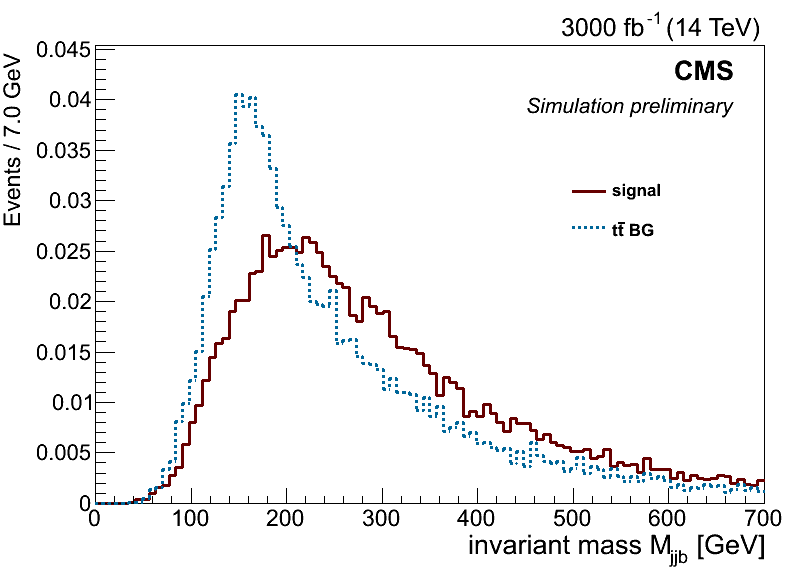
\includegraphics[width=\ww]{figs/M_jjb.png}
    \end{minipage}
    \hspace{9mm}
  \end{subfigure}	
  \vspace{\dd}
  \caption{Variables distribution of HH (red) and \tt\ (blue) for the neural network: Higgs mass reconstructions $M_{\b\b}$ and $M_{jj\ell\nu}$ and top mass reconstructions $M_{jj\text{b}_1}$ and $M_{\text{b}_2\text{\lnu}}$.} \label{vars7}

\end{figure*}




% FIGURE: M b2l, j1l and MT
\begin{figure*}[h]
	
  % SUBFIGURES
  \begin{subfigure}[b]{17cm}
    % fig a
    \begin{minipage}[h!]{\ww}
      \centering
      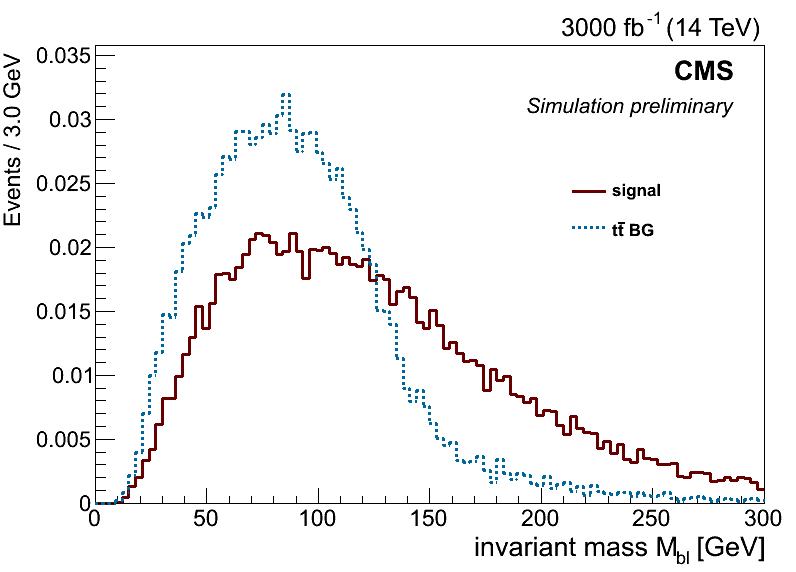
\includegraphics[width=\ww]{figs/M_bl.png}
    \end{minipage}
%    \hspace{\w}
    % fig b
    \begin{minipage}[h!]{\ww}
      \centering
      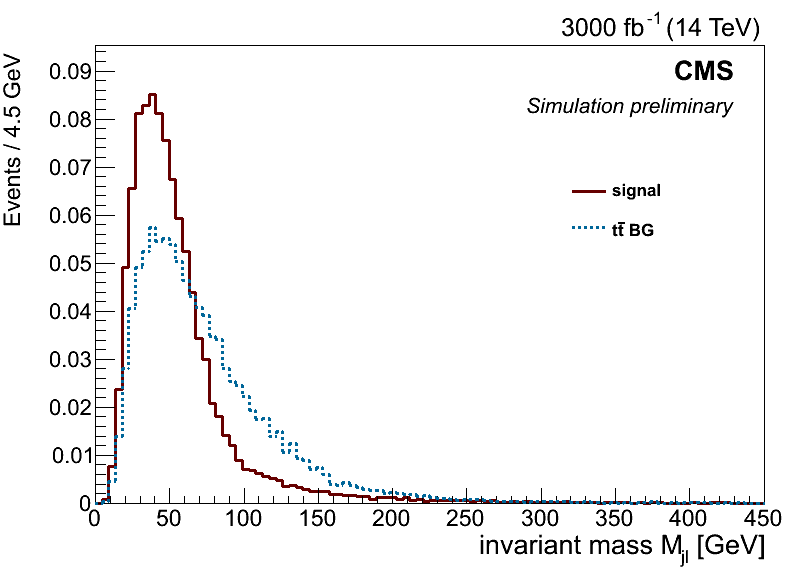
\includegraphics[width=\ww]{figs/M_j1l.png}
    \end{minipage}
  \end{subfigure}

  % SUBFIGURES
  \begin{subfigure}[b]{17cm}
%    % fig a
%    \begin{minipage}[h!]{\ww}
%      \centering
%      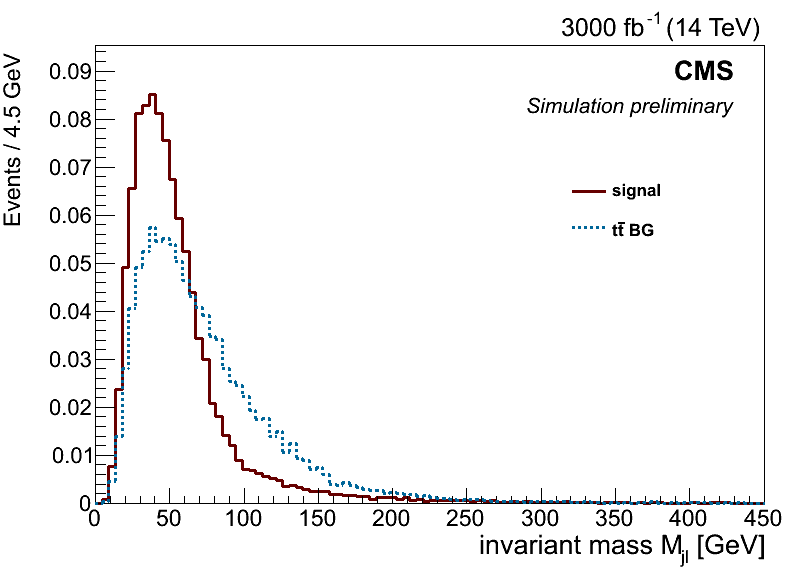
\includegraphics[width=\ww]{figs/M_j1l.png}
%    \end{minipage}
%%    \hspace{\wb}
    % fig b
%    \begin{minipage}[h!]{\ww}
      \centering
      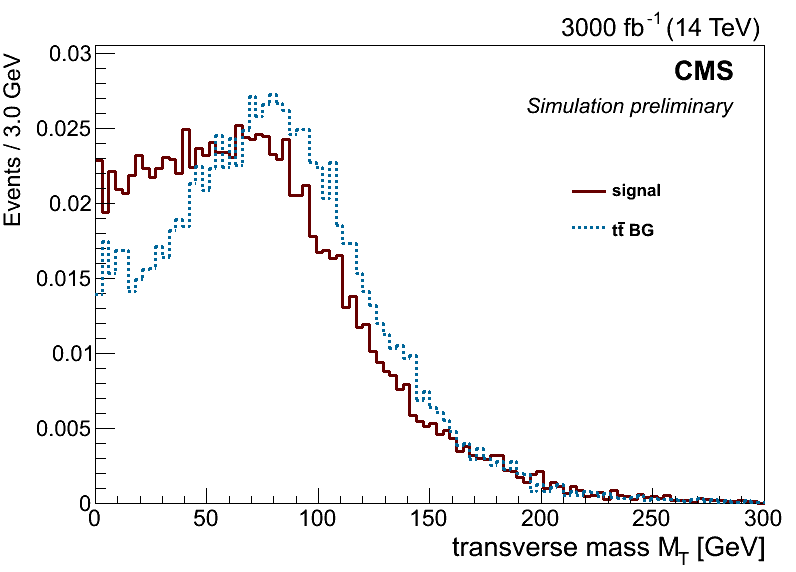
\includegraphics[width=\ww]{figs/MT_lnu.png}
%    \end{minipage}
%    \hspace{9mm}
  \end{subfigure}	
  \vspace{\dd}
  \caption{Variables distribution of HH (red) and \tt\ (blue) for the neural network: $M_{\text{b}_2\text{\l}}$ and $M_T^{\ell\nu}$ (see Eq. \eqref{MT}).} \label{vars8}

\end{figure*}



% FIGURE: MVA output
\begin{figure*}[h] 
	
    % fig a
    \begin{minipage}[h!]{\ww}
      \centering
      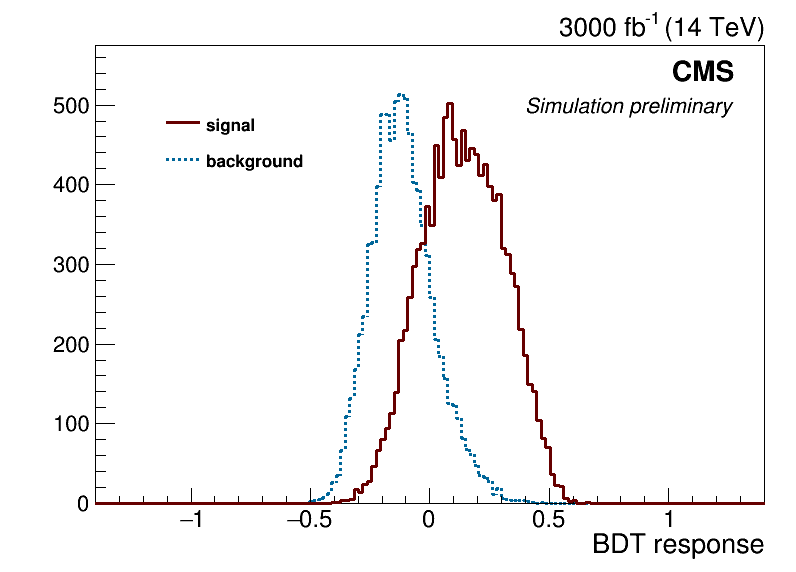
\includegraphics[width=\ww]{figs/BDTBoost1_everything4CleanUp.png}
    \end{minipage}
%    \hspace{\w}
    % fig b
    \begin{minipage}[h!]{\ww}
      \centering
      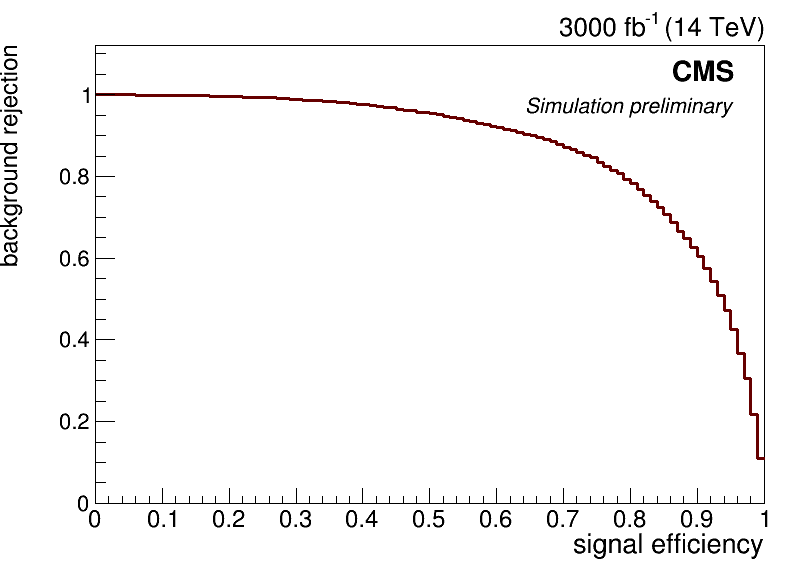
\includegraphics[width=\ww]{figs/BrejvsSeffs_everything4CleanUp_BDTBoost1.png}
    \end{minipage}
  \caption{Final BDT output and background rejection versus signal efficiency.} \label{BDT}

\end{figure*}








% References
\begin{thebibliography}{1}

\bibitem{AN} C. Delaere \etal, \emph{Study of HH production with H $\rightarrow$ bb, H $\rightarrow$ WW $\rightarrow \ell\nu\ell\nu$ for an upgraded CMS detector at the HL-LHC}, CMS draft analysis note 2014/141.

\bibitem{sigma_HH} D. de Florian \& J. Mazzitelli, \emph{Higgs Boson Pair Production at Next-to-Next-to-Leading Order in QCD}. Phys. Rev. Lett. \textbf{111} (Nov, 2013) 201801, \href{http://journals.aps.org/prl/abstract/10.1103/PhysRevLett.111.201801}{\texttt{doi:10.1103/PhysRevLett.111.201801}}, \href{http://arxiv.org/abs/1309.6594}{\texttt{arXiv:1309.6594}}.

\bibitem{sigma_tt} \emph{NNLO+NNLL top-quark-pair cross sections - ATLAS-CMS recommended predictions for top-quark-pair cross sections using the Top++v2.0 program (M. Czakon, A. Mitov, 2013)}, \url{https://twiki.cern.ch/twiki/bin/view/LHCPhysics/TtbarNNLO#Top_quark_pair_cross_sections_at}.

\bibitem{sigma_HH_NLO} R. Frederix \etal, \emph{Higgs pair production at the LHC with NLO and parton-shower effects}, Phys. Rev. Lett. \textbf{B723} (May, 2014) 142, \href{http://dx.doi.org/10.1016/j.physletb.2014.03.026}{\texttt{doi:10.1016/j.physletb.2014.03.026}}, \href{http://link.aps.org/doi/10.1103/PhysRevLett.112.221801}{\texttt{arXiv:1401.7340}}.

\bibitem{BR_HH} \emph{Higgs cross sections for European Strategy studies in 2012}, \url{https://twiki.cern.ch/twiki/bin/view/LHCPhysics/HiggsEuropeanStrategy2012#SM_Higgs_decay_branching_ratio_M}.

%\bibitem{BR_tt} K.A. Olive \etal (Particle Data Group), Chin. Phys. \textbf{C38}, 090001 (014) (\url{http://pdg.lbl.gov/2014/tables/rpp2014-sum-quarks.pdf}.

\bibitem{BR_tt} T. Aaltonen \etal\ (CDF Collaboration), \emph{Measurement of $\mathcal{B}(\text{t $\rightarrow$ Wb}) / \mathcal{B}(\text{t $\rightarrow$ W$q$})$ in Top-Quark-Pair Decays Using Dilepton Events and the Full CDF Run II Data Set}, Phys. Rev. Lett. \textbf{112}, 221801 (June, 2014), \href{http://journals.aps.org/prl/abstract/10.1103/PhysRevLett.112.221801}{\texttt{doi:10.1103/PhysRevLett.112.221801}}, \href{http://arxiv.org/abs/1404.3392}{\texttt{arXiv:1404.3392}}.

\bibitem{BR_W} J. Beringer \etal\ (Particle Data Group), PR \textbf{D86}, 010001 (2012) and 2013 partial update for the 2014 edition (\url{http://pdg.lbl.gov/2013/listings/rpp2013-list-w-boson.pdf}).

%\bibitem{code_HH} I. Neutelings (Oct, 2015), \url{https://github.com/IzaakWN/Delphes/blob/IzaakFall2015/python/HHEventSelection_dilep.py}
%
%\bibitem{code_tt} I. Neutelings (Oct, 2015), \url{https://github.com/IzaakWN/Delphes/blob/IzaakFall2015/python/ttEventSelection_dilep.py}

\end{thebibliography}




% _BRANCHINGRATIOS_HIGGS_BOSON_
%
% https://twiki.cern.ch/twiki/bin/view/LHCPhysics/HiggsEuropeanStrategy2012#SM_Higgs_decay_branching_ratio_M
%    BR(H->bb) = 0,577
%    BR(H->WW) = 0,215
%    BR(H->ZZ) = 0,0264



% _BRANCHINGRATIOS_W_AND_Z_BOSONS_
%
% http://pdg.lbl.gov/2013/listings/rpp2013-list-w-boson.pdf
%    BR(W->qq) = 0,6760
%    BR(W->ev) = 0,1075
%    BR(W->muv) = 0,1057
%    BR(W->tauv) = 0,1125
%
% http://pdg.lbl.gov/2014/listings/rpp2014-list-z-boson.pdf
%    BR(Z->qq) = 0,6991
%    BR(Z->ll) = 0,0337
%    BR(Z->vv) = 0,20/3 = 0,066 ?
%
% Without taus:
%    BR(WW->lvlv) = 0,1075^2 + 2*0,1075*0,1057 + 0,1057^2 = ~ 0,0455
%                 = 4*0,1080^2 = 0,047   % average values
%                 = 4*0,11^2 = 0,0484    % rounded values
%    BR(WW->qqlv) = 2*0,676*(0,1075 + 0,1057)
%                 = 0,2882464 ~ 0,2883
%
% With taus:
%    BR(WW->lvlv) = 0,1075^2 + 0,1057^2 + 0,1125^2
%                   + 2*0,1075*0,1057 + 2*0,1075*0,1125 + 2*0,1057*0,1125
%                 = 0,10608049 ~ 0,1061
%    BR(WW->qqlv) = 2*0,676*(0,1075 + 0,1057 + 0,1125)
%                 = 0,4403464 ~ 0,4403



% _BRANCHINGRATIOS_HH_
%
% Without taus:
%    BR(HH->bbWW->bblvlv) = 2*BR(H->bb)*BR(H->WW)*BR(W->lv)^2
%                         = 2*(0,215*0,577)*(0,1075^2 + 2*0,1075*0,1057 + 0,1057^2)
%                         = 0,01127765149 ~ 0,0113
%    BR(HH->bbWW->bbqqlv) = 2*BR(H->bb)*BR(H->WW)*2*BR(W->qq)*BR(W->lv)
%                         = 2*(0,215*0,577)*2*0,676*(0,1075 + 0,1057)
%                         = 0,0715168143 ~ 0,0715
%
% With taus:
%    BR(HH->bbWW->bblvlv) = 2*BR(H->bb)*BR(H->WW)*BR(W->lv)^2
%                         = 2*(0,215*0,577)*( 0,1075^2 + 0,1057^2 + 0,1125^2
%                           + 2*0,1075*0,1057 + 2*0,1075*0,1125 + 2*0,1057*0,1125 )
%                         = 0,02631963037 ~ 0,0263
%    BR(HH->bbWW->bbqqlv) = 2*BR(H->bb)*BR(H->WW)*2*BR(W->qq)*BR(W->lv)
%                         = 2*(0,215*0,577)*2*0,676*(0,1075 + 0,1057 + 0,1125)
%                         = 0,1092543453 ~ 0,1093
%
% Sample with only H->bb, H->WW combinations
%    2*(0,577)*(0,215) / (2*(0,577)*(0,215)+(0,577)^2+(0,215)^2) ~ 0,3955
%      (0,577)^2 / (2*(0,577)*(0,215)+(0,577)^2+(0,215)^2) ~ 0,5308
%      (0,215)^2 / (2*(0,577)*(0,215)+(0,577)^2+(0,215)^2) ~ 0,0737
%
%



% _BRANCHINGRATIOS_tt_
%
% http://arxiv.org/pdf/1404.3392.pdf
% http://pdg.lbl.gov/2014/reviews/rpp2014-rev-top-quark.pdf
% http://pdg.lbl.gov/2014/tables/rpp2014-sum-quarks.pdf
%    BR(t->bW) = 0,99830 CDF 2014
%    BR(t->bW) = 0,91 PDG 2014
%
% Without taus
%    BR(tt->bbWW->bblvlv) = 0,99830^2 * (0,1075^2 + 2*0,1075*0,1057 + 0,1057^2)
%                         = 0,04529982695 ~ 0,0453 CDF
%                         = 0,03764065614 ~ 0,0377 PDG
%    BR(tt->bbWW->bbqqlv) = 0,99830^2 * 2*0,676*(0,1075 + 0,1057)
%                         = 0,2872671953 ~ 0,2873 CDF
%                         = 0,2386968438 ~ 0,2387 PDG
%
% With taus
%    BR(tt->bbWW->bblvlv) = 0,99830^2 * ( 0,1075^2 + 0,1057^2 + 0,1125^2
%                           + 2*0,1075*0,1057 + 2*0,1075*0,1125 + 2*0,1057*0,1125 )
%                         = 0,1057201229 ~ 0,1057
%    BR(tt->bbWW->bbqqlv) = 0,99830^2 * 2*0,676*(0,1075 + 0,1057 + 0,1125)
%                         = 0,4388504948 ~ 0,4389



% 0,163*2,3/0.0113 = 33,177
% 18899/50789 = 0,372
% 9030*1,85/0,0454/0,37 = 994493
% 9030*1,85/0,37/984500 = 0,04586

% (40*0,0113*3000)*.../51464/(1+sqrt(984500*0,0453*3000*.../50789))
% (40*0,0113*3000)*.../51464/(1+sqrt(984500*0,0453*3000*.../18899))
% (40*0,0715*3000)*.../214888/(1+sqrt(984500*0,2873*3000*.../211952))
% (40*0,0715*3000)*.../214888/(1+sqrt(984500*0,2873*3000*.../182709))
% (0,163*2,3*3000)*.../51464/(1+sqrt(9030*1,85*3000*.../18899))
% (0,163*2,3*3000*715/113)*.../214888/(1+sqrt(9030*1,85*3000*2873/453*.../182709))

%           S = 979907  B = 499600
% stage_0:  S = 51464   B = 50789
% stage_1:  S = 51464   B = 18899
% stage_2:  S = 3181    B = 2023
% stage_3:  S = 2499    B = 331
% stage_4:  S = 214888  B = 211952
% stage_5:  S = 214888  B = 182709
% stage_6:  S = 26511   B = 35223
% stage_7:  S = 20634   B = 15335



\end{document}
